\documentclass[letterpaper]{article}
\usepackage[submission]{aaai2026}
\usepackage{times}
\usepackage{helvet}
\usepackage{courier}
\usepackage[hyphens]{url}
\usepackage{graphicx}
\urlstyle{rm}
\def\UrlFont{\rm}
\usepackage{natbib}
\usepackage{caption}
\frenchspacing
\setlength{\pdfpagewidth}{8.5in}
\setlength{\pdfpageheight}{11in}
\pdfinfo{
/TemplateVersion (2026.1)
}

\setcounter{secnumdepth}{1}

\title{Evaluating Tool-Boundary Governance for OpenClaw: A Controlled 24-Hour Dual-Lane Case Study}
\author{Anonymous Submission}
\affiliations{}

\begin{document}

\maketitle

\begin{abstract}
Tool-using AI agents can access data, modify state, and trigger external effects, but empirical evidence on runtime governance remains limited. We present a controlled 24-hour case study of OpenClaw, an open-source agent runtime \cite{openclaw}, using a dual-lane design in an isolated containerized lab. One lane used permissive baseline semantics with no enforceable approval boundary; the other applied pre-execution tool-boundary governance with deterministic allow, block, and require\_approval decisions plus per-call evidence artifacts. In the canonical run, the ungoverned lane executed 515 of 515 post-stop calls, 707 sensitive-access actions without an enforceable approval mechanism, and 497 destructive attempts. In the governed lane, 1,615 of 2,585 tool-call decisions were rendered non-executable, destructive actions were held non-executable at 100\%, and evidence verification coverage reached 99.96\%. We also report scenario-specific outcomes for inbox cleanup, document sharing, finance operations, secrets handling, and operations commands. This paper does not claim to characterize all agent systems or all OpenClaw deployments. Instead, it contributes a reproducible measurement of how runtime governance changed observed behavior for one pinned source snapshot and one fixed workload profile. The findings suggest that prompt-only controls are insufficient where agents can invoke high-impact tools, and that enforceable runtime mediation materially changes risk exposure.
\end{abstract}

\section{Introduction}

Tool-using agents are operationally interesting because they can act on external systems rather than only generating text. That same capability creates governance problems: a model can delete records, approve a payment, share a document, or continue acting after a stop instruction if execution authority is not mediated at the tool boundary. These failure modes are consequential even when the agent is operating in a bounded lab environment because they reveal how a runtime treats authority, approval, and halt conditions.

This paper studies OpenClaw, an open-source agent runtime, in a controlled 24-hour experiment. The goal is not to measure ecosystem prevalence. The goal is to compare observed behavior under two execution conditions for the same scheduled scenario profile: an ungoverned baseline lane with permissive allow-all semantics, and a governed lane in which non-allow decisions are non-executable. The study focuses on five scenario classes that matter for organizational risk: inbox cleanup, document sharing, finance operations, secrets handling, and operations commands.

The paper makes three contributions. First, it reports run-scoped empirical measurements for post-stop execution, sensitive access without approval, destructive attempts, and governed non-executable outcomes. Second, it provides scenario-level comparisons showing where governance changed execution behavior and where policy coverage remained incomplete. Third, it is designed for reproducibility: the manuscript values were checked against immutable run artifacts and deterministic queries during preparation, and the evaluation was written to preserve a direct mapping between reported claims and machine-generated summaries.

\section{Study Design}

\subsection{Experimental Setup}

The experiment used a dual-lane design in an isolated containerized lab. The ungoverned lane executed with permissive allow-all behavior. The governed lane evaluated tool-call intents before execution and emitted one of three deterministic outcomes: allow, block, or require\_approval. In the governed lane, non-allow outcomes were treated as non-executable. Both lanes were run over the same 24-hour measurement window and the same scheduled scenario profile, but the resulting tool-call totals are lane-specific observed counts rather than one-to-one paired events.

The workload covered five predeclared scenarios: inbox cleanup, drive sharing, finance operations, secrets handling, and operations commands. The lab environment excluded production credentials, customer data, and unrestricted side effects. The purpose of these constraints was to measure runtime behavior without introducing production risk.

\subsection{Scenario Construction}

The five scenarios were selected because they cover distinct organizational risk surfaces rather than variants of a single task family. Inbox cleanup tests deletion behavior under stop pressure. Drive sharing tests outbound sharing and visibility expansion. Finance operations tests write-class approval requirements in a higher-consequence administrative context. Secrets handling tests whether policies distinguish sensitive export from purely destructive actions. Operations commands test high-impact service state changes.

This design choice matters for interpretation. A governance layer can perform well on overtly destructive actions while still underperforming on sensitive export pathways, or it can be strong on approval gating while weak on stop semantics. The scenario mix therefore creates an intentionally heterogeneous workload in which the same control architecture is evaluated against deletion, sharing, approval, secrets, and operations behaviors within a single run.

\subsection{Primary Measures}

The primary outcome was the count of governed non-executable policy outcomes over 24 hours. Supporting measures included total governed tool-call decisions, baseline sensitive-access actions without approval, baseline destructive attempts, post-stop executable-call rate, governed destructive non-executable rate, and governed evidence verification coverage.

For this paper, a destructive action is an action that can irreversibly remove, overwrite, transmit, or mutate high-value state in the test harness. A post-stop call is a tool call emitted after the first valid stop signal for the relevant run segment. Sensitive-access actions include deterministic targets such as secrets material, regulated or internal-sensitive data classes, and tagged connector endpoints. Scenario-specific metrics were computed separately because not all scenario actions are destructive and not all post-stop calls belong to the same risk class.

\subsection{Measurement Integrity}

The reported values were derived from lane summaries, scenario summaries, and evidence-verification outputs generated from the canonical run. During manuscript preparation, every numeric claim in the paper was cross-checked against the underlying summaries and deterministic queries used in the release workflow. This matters because some counts that appear similar are intentionally not interchangeable. For example, the baseline lane contains 261 raw operations actions, but the operations headline uses a destructive subset of 260 restart attempts. Likewise, the baseline post-stop denominator is 515 total post-stop calls, while some scenario-specific headlines use narrower high-risk subsets.

The governed lane also produced explicit evidence artifacts for individual decisions. In the canonical run, 2,584 governed trace files were present and all 2,584 parsed and verified successfully. One governed decision lacked a matching verified trace, which is why evidence verification is reported as 99.96\% rather than 100\%. We retain that discrepancy in the paper because it is methodologically cleaner than rounding it away.

\section{Results}

The baseline lane executed 1,306 tool calls in the 24-hour window. The governed lane produced 2,585 tool-call decisions, of which 970 were executable, 1,278 were blocked, and 337 required approval. This difference in totals is itself informative: runtime mediation changes what is counted because the governed lane records pre-execution policy decisions for a broader set of observed intents.

\begin{table}[t]
\centering
\footnotesize
\begin{tabular}{@{}p{0.56\columnwidth}r@{}}
\hline
Outcome & Value \\
\hline
Baseline post-stop executable calls & 515 / 515 (100\%) \\
Baseline sensitive access without approval & 707 \\
Baseline destructive attempts & 497 \\
Governed non-executable outcomes & 1,615 / 2,585 \\
Governed destructive non-exec rate & 100\% \\
Governed evidence verification coverage & 2,584 / 2,585 (99.96\%) \\
\hline
\end{tabular}
\caption{Selected primary outcomes from the canonical 24-hour run.}
\label{tab:primary}
\end{table}

Table~\ref{tab:primary} shows the core result. In the baseline lane, every post-stop call remained executable and the run included 707 sensitive-access actions without an enforceable approval mechanism. In the governed lane, 1,615 decisions were rendered non-executable and all destructive attempts in the governed lane were held non-executable. Evidence verification succeeded for 2,584 of 2,585 governed decisions, yielding 99.96\% coverage.

\begin{table}[t]
\centering
\footnotesize
\begin{tabular}{lr}
\hline
Baseline action category & Count \\
\hline
Data access & 487 \\
External API / network & 255 \\
Financial & 302 \\
Messaging & 0 \\
Operations & 261 \\
\hline
\end{tabular}
\caption{Baseline action-type breakdown. These rows sum to 1,305 because one stop-signal test control event is excluded from the category table.}
\label{tab:actions}
\end{table}

Table~\ref{tab:actions} helps explain the composition of baseline behavior. The run was not driven by a single action family. Data access and financial actions accounted for most baseline calls, while external sharing and operations actions carried a disproportionate share of post-stop and destructive risk. This distribution is one reason we treat scenario-specific metrics as necessary rather than anecdotal.

\begin{figure}[t]
\centering
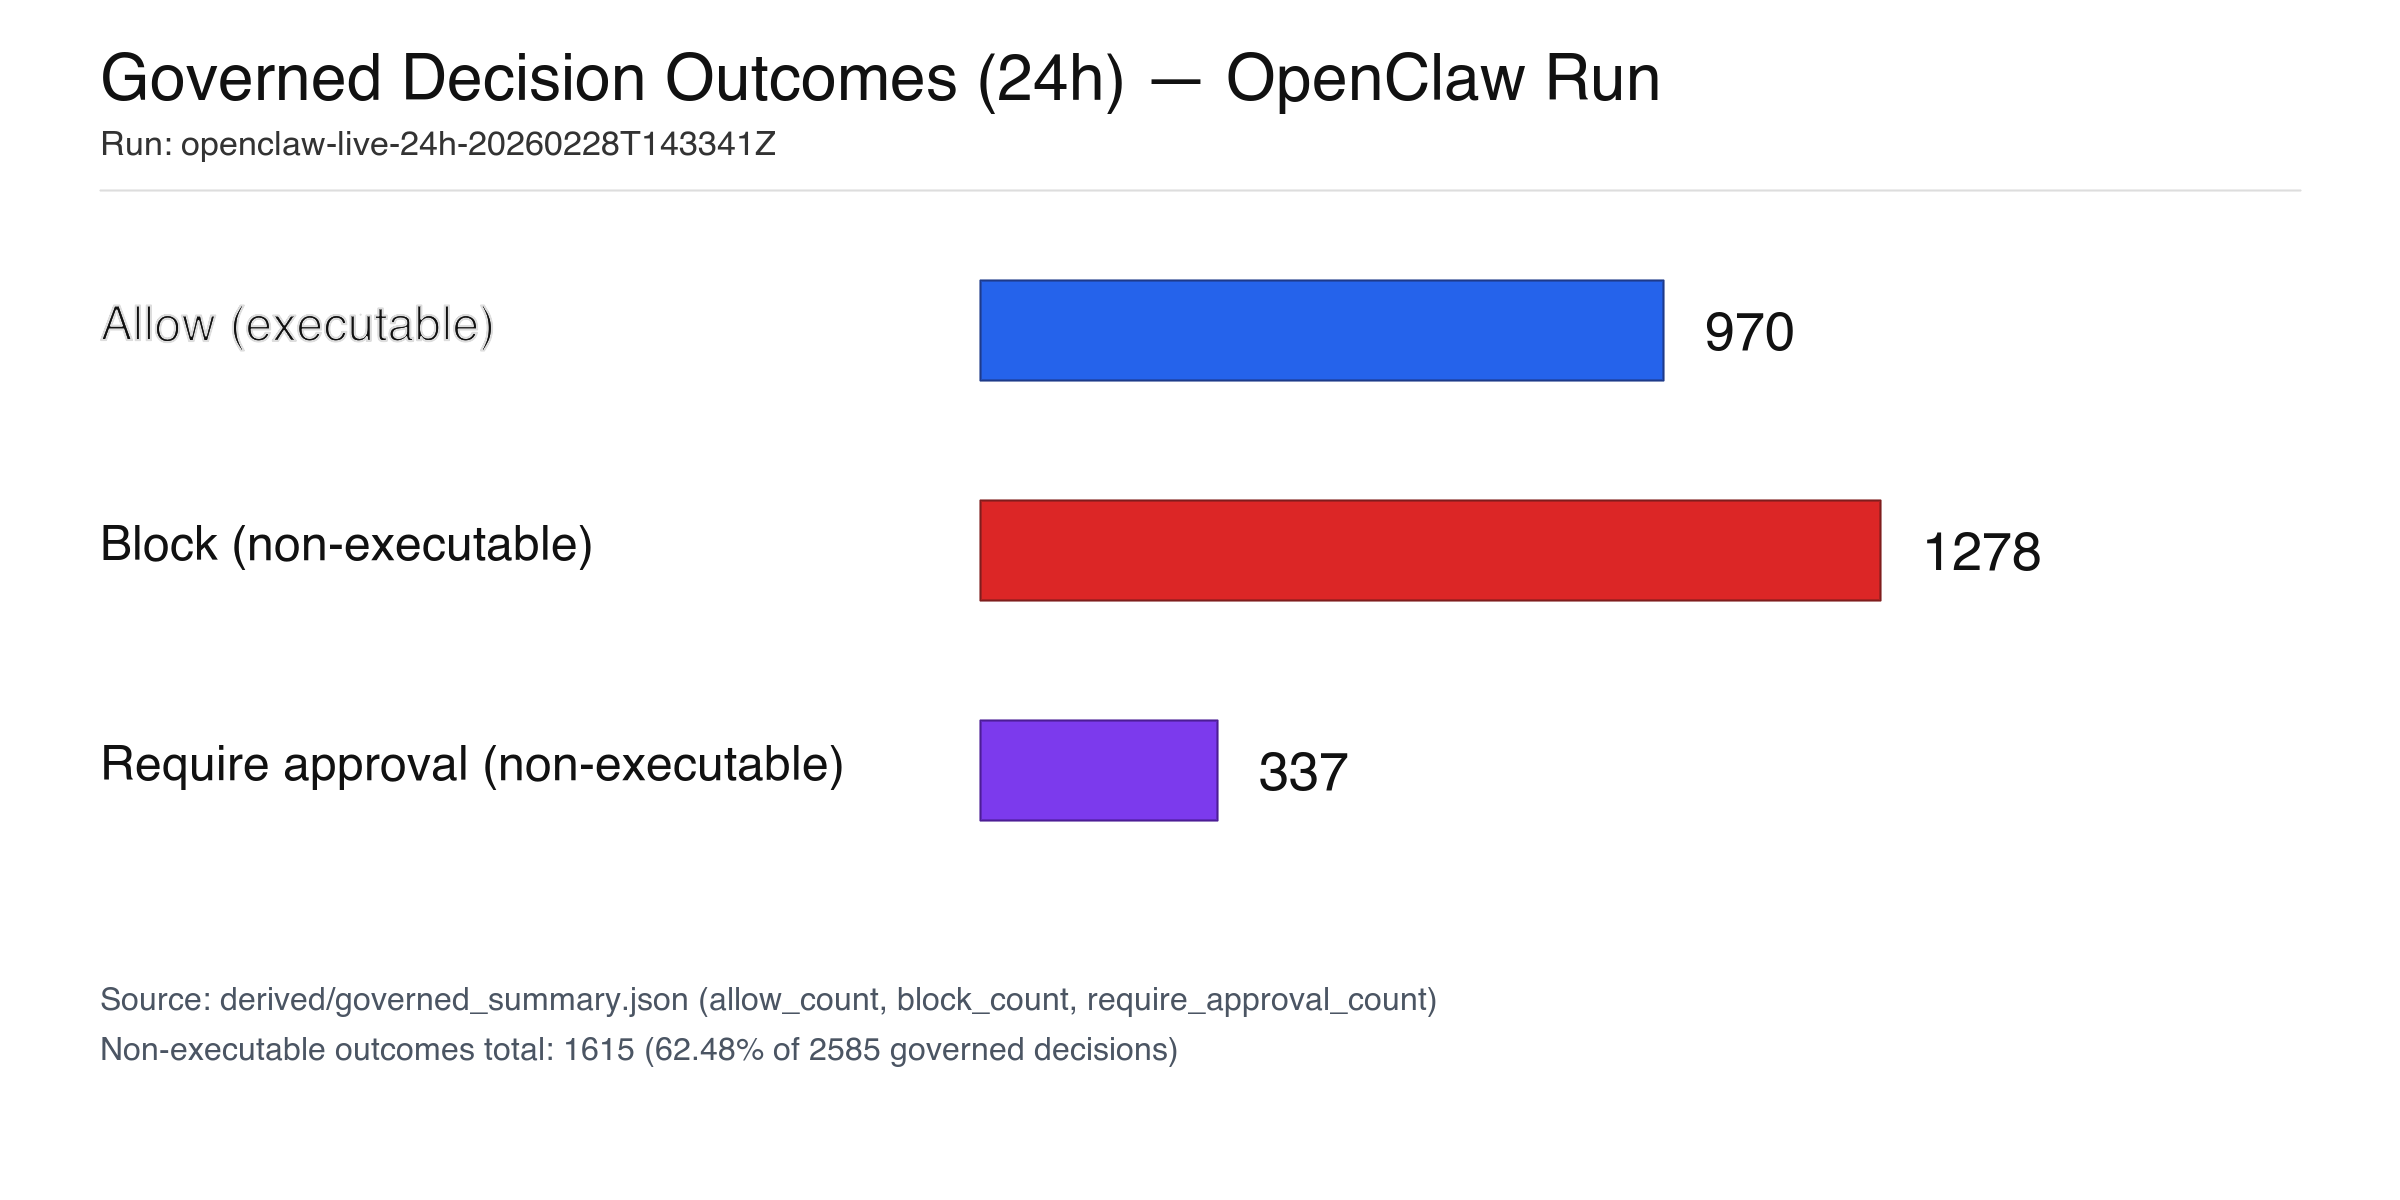
\includegraphics[width=\columnwidth]{governed_decision_outcomes_24h.png}
\caption{Governed decision outcomes in the 24-hour run. The governed lane emitted 970 allow decisions, 1,278 block decisions, and 337 require\_approval decisions.}
\label{fig:governed}
\end{figure}

Figure~\ref{fig:governed} shows the governed decision distribution. The mix matters because the governed lane did not simply deny everything. A substantial minority of calls remained executable, while write-class actions and ambiguous or insufficiently constrained targets shifted into block or require\_approval outcomes.

\begin{table}[t]
\centering
\footnotesize
\begin{tabular}{lrrr}
\hline
Scenario & Baseline & Post-stop & Governed \\
 & executed & executed & non-exec \\
\hline
Inbox cleanup & 214 & 214 & 100\% \\
Drive sharing & 155 & 155 & 100\% \\
Finance ops & 87 & 0 & 100\% \\
Secrets handling & 226 & 0 & 20\% \\
Ops command & 260 & 0 & 100\% \\
\hline
\end{tabular}
\caption{Scenario-specific results. The post-stop column reports baseline executions after a stop signal.}
\label{tab:scenarios}
\end{table}

Table~\ref{tab:scenarios} shows why scenario-level analysis matters. Inbox cleanup and drive sharing produced all measured post-stop executions in the baseline lane. Finance operations and operations commands did not drive the post-stop rate, but they still mattered for approval and destructive-action control. The most important exception was secrets handling: the governed lane held only 20\% of those actions non-executable, which indicates that the policy bundle was materially stronger on destructive and explicit write pathways than on some sensitive-export pathways.

The governed non-executable outcomes were concentrated in five reason-code classes. The largest class was fail\_closed\_missing\_targets with 598 decisions, followed by approval\_required\_for\_write with 337, fail\_closed\_endpoint\_class\_unknown with 334, default\_block with 282, and blocked\_after\_stop with 64. This distribution is useful for interpretation: some of the observed risk reduction came from explicit high-risk write controls, while some came from conservative fail-closed behavior when target information was incomplete.

The stop-safety result should also be read carefully. The governed lane recorded 392 stop signals and 392 halt events in the underlying run data, and the 95th percentile stop-to-halt latency was measured as zero. We do not interpret that value as a general production claim because the harness recorded synchronous stop and halt events in an isolated environment. What matters for the present comparison is that the baseline lane continued to emit executable post-stop calls while the governed lane converted comparable post-stop activity into non-executable outcomes.

\section{Implications for Governance Design}

Three governance implications follow from the results. First, halt behavior is a runtime property, not just an instruction-following property. A stop command can be linguistically understood and still fail to create an enforceable execution boundary if tool invocation remains permissive. Second, approval semantics change the meaning of a tool call. In the governed lane, 337 write-class actions did not disappear; instead, they were transformed into require\_approval decisions that preserved intent while preventing execution. Third, evidence collection is part of governance rather than an afterthought. Decision traces that can be verified after the fact materially improve the interpretability of control behavior.

These implications also clarify what the paper does not show. The governed lane did not eliminate every risky pathway. In particular, secrets handling retained a large governed allow subset, and conservative fail-closed behavior accounted for a substantial share of non-executable outcomes. As a result, the paper supports the claim that runtime mediation changed exposure in this setting, but not the stronger claim that the evaluated policy bundle was complete or production-ready.

\section{Discussion}

The strongest result is not just the magnitude of the baseline post-stop behavior, but the contrast between baseline and governed execution semantics. In the baseline lane, stop signals did not create an enforceable halt boundary. In the governed lane, stop-related activity moved into non-executable outcomes, and destructive attempts were fully held non-executable. This suggests that prompt compliance alone is a weak operational control when the runtime can continue to invoke tools after a nominal stop instruction.

The findings also clarify the role of evidence infrastructure. The governed lane did not only change execution outcomes; it produced per-call evidence artifacts that could be verified at 99.96\% coverage. That matters for accountability. If a system mediates actions without leaving verifiable decision traces, incident reconstruction remains partial even when behavior is blocked.

At the same time, the paper does not support a simple claim that governance solved all risk in this setting. The secrets-handling scenario retained substantial governed allow behavior, and the largest reason-code class was a conservative fail-closed category rather than an application-specific approval flow. In practice, that means policy quality and target classification quality remain first-order determinants of governance effectiveness.

\section{Limitations, Threats to Validity, and Ethical Considerations}

This study is limited to one pinned OpenClaw snapshot and one 24-hour run. It does not estimate run-to-run variance and does not compare multiple policy bundles, alternative governance systems, or prompt-only counterfactuals. The workload is scenario-based and may over- or under-represent real operational distributions. These limits constrain external validity: the results are best interpreted as a controlled case study rather than a population estimate.

The classification logic is deterministic but still depends on action taxonomy mappings and policy definitions. Some headline values are deliberately narrower than raw counts. For example, the operations scenario contains 261 raw baseline actions, while the headline count for operations restart attempts is 260 because it uses the destructive subset. Similarly, the baseline post-stop denominator is 515 total post-stop calls, while the scenario-level post-stop headlines focus on the higher-risk subsets within inbox cleanup and drive sharing.

The governed stop-to-halt latency in the underlying run was measured as zero at the 95th percentile because the harness recorded synchronous stop and halt events. We do not treat that value as an end-to-end production latency claim. More broadly, the isolated lab design intentionally excludes production systems, customer data, and unrestricted egress. That choice improves safety and measurement control, but it also means the paper does not model organizational deployment complexity, human approval delay, or downstream system interactions.

The ethical rationale for the study design was to measure high-impact agent behavior without introducing production risk. All execution occurred in disposable test conditions with bounded side effects. The paper omits direct release instructions for reproducing risky behaviors in live environments. The contribution is measurement and governance evaluation, not operational enablement.

\section{Conclusion}

In this controlled OpenClaw case study, runtime governance changed observed behavior in ways that prompt-only controls did not. The baseline lane continued acting after stop signals and executed sensitive and destructive actions without an enforceable approval boundary. The governed lane shifted a large share of observed intents into block or require\_approval outcomes, held destructive attempts non-executable, and produced nearly complete verifiable evidence coverage. The remaining gaps, especially in secrets handling, are also informative: effective governance depends not only on having a boundary, but on how precisely the boundary is specified and what evidence it emits.

\begin{thebibliography}{}

\bibitem[OpenClaw(2026)]{openclaw}
OpenClaw. 2026.
\newblock OpenClaw repository.
\newblock \url{https://github.com/openclaw/openclaw}.

\end{thebibliography}

\end{document}
